\chapter{Concepts}
\label{chapter:concepts}

We introduce the important concepts required for the thesis in this chapter.

\section{Paxos}
\label{section:concepts.paxos}

\subsection{Terminology}

\begin{itemize}
    \iterm{Proposal}: A request sent by the client that is to be executed on all
    the nodes in the cluster.
    \iterm{Decision}: A proposal that is successfully agreed upon by the
    cluster.
    \iterm{Master Leader}: The leader process running on the master node.
    \iterm{Master Replica}: The replica process running on the master node.
    \iterm{Slot}: Each of the decisions are discrete events. The events can be
    mapped to a log file. The indices of the transaction log file are termed
    \term{slot}s.
    \iterm{Node}: An independent Erlang runtime instance.
    \iterm{Membership}: The nodes in the cluster are called members. They can be
    a member of different groups based on their condition%
    \sidenote{
      The condition of the node is a reference to the node's status in terms of
      handling the algorithm. Possible conditions are
      \begin{inparaenum}[(i)]
        \iterm{Valid}: A node that is ready to handle the messages and take part
        in the protocol.
        \iterm{Join}: A fresh node that is in the process of joining the
        cluster.
        \iterm{Down}: A node that was once a part of the cluster, but is
        currently inaccessible is moved to this state until it can be fixed
        manually.
      \end{inparaenum}
    }.
    \term{join}
    \iterm{Master}: The node that is elected and is the only one who can handle
    proposals sent by the replica.
    \iterm{Lease}: The master node retains its status as master for the duration
    of the lease. Lease time dictates the maximum possible time for which data
    read could be stale.
\end{itemize}

\subsection{Algorithm}

We use Paxos \sectionref{paxos} as the consensus algorithm for the system.
\citet{Robbert2011}'s \val{Paxos Made Moderately Complex} is the specific paper
referred to for the implementation of
Warlock. Firstly, we use this specific flavour since the detailed pseudo code
specified maps very well to the Erlang's process oriented%
\sidenote{
  Erlang uses light weight processes for concurrency. These processes
  communicate using messages.
} design. Secondly, the paper discusses multiple optimizations required to make
the algorithm practical.

The processes of the group can be classified into different roles based on the
part of algorithm they are responsible for.

\begin{itemize}
    \iterm{Replica}: Replicas are processes responsible for assigning a proposal
    number to an operation and handle decisions received.
    \iterm{Acceptor}: Acceptors are the \val{memory} of the algorithm. They keep
    track of which leader is currently in-charge to issue commands using
    ballots%
    \sidenote{
      \emph{Ballots} are monotonically increasing identifiers that are unique to
      a specific leader. Each leader has an infinite number of ballots.
    }.
    \iterm{Leader}: Leaders receive proposals from replicas and they try to
    co-ordinate the messaging to acceptors for that proposal. It uses ballots
    to track the execution order of proposals.
    \iterm{Scout}: A scout process is spawned by the leader to active a specific
    ballot.
    \iterm{Commander}: A commander process is spawned by the leader to try
    and get votes for a specific proposal.
\end{itemize}

Assuming the scout was already run and the current leader has its ballot as the
largest one, lets see a typical flow of the proposal from its initiation to its
execution skipping on the smaller details and corner cases.

\begin{enumerate}
    \item A proposal is created by the client based on the request. This
      proposal is uniquely identified and contains the complete request
      information. This proposal is sent to the replica.
    \item The replica checks if the proposal is a duplicate and if not it
      assigns a sequence number%
      \sidenote[-2]{
        The replica is responsible for maintaining a consistent log of
        operations. This log is made up of slots with each of the slots
        indexed by a sequence number.
      }
      to it before sending it off to the leader.
    \item The leader, which already has run the scout, spawns a commander with
      the ballot and proposal information.
    \item The commander sends out a message to all acceptors with the ballot
      information to all acceptors asking them to approve the proposal.
    \item The acceptor respond positively if it has not seen a larger
      ballot and negatively otherwise.
    \item The commander waits for a quorum (usually a majority of total
      acceptors). Once it has received majority of the approvals,
      the commander asks all the replicas to execute the proposal and exits.
    \item The replica checks if the received decision is the next index on
      the consistent log and executes the proposal if it is.
\end{enumerate}

The above use case constitutes a single Paxos instance among a set of processes.
In general, the system may consists of several of these processes running
concurrently. In this scenario, the routing works as follows.

\begin{enumerate}
  \item The client broadcasts its command to all the replicas.
  \item Each of the replica sends a \term{propose} message to all the leaders.
  \item The leader sends the \code{P1A} message to all the acceptors via the 
    scout.
  \item The acceptor only replies to the sender with a \code{P1B} message.
  \item On quorum acceptance from a quorum of acceptors, the leader sends
    \code{accept} message (\code{P2A}) to all the acceptors via the commander.
  \item The acceptors responds with \code{P2B} only to the sender.
  \item The leader on quorum response, broadcasts the decision to all the
    replicas.
  \item Each of the replica replies to the client.
\end{enumerate}

The paper details a few optimizations for state reduction and improving
performance, making the implementation more practical. It also offers
several suggestions from the implementation and deployment perspective.

\section{Erlang}

Erlang \citep{erlang} is a general purpose functional
programming%
\sidenote{
  \emph{Functional Programming}: is where programs are run by evaluating
  expressions as opposed to imperative programming where statements are run
  to change state. The data used in this type of programming is typically
  not mutable.
} language built by Ericsson mainly to develop telephony applications
\citep{Armstrong07}. Erlang was build to handle large number of network
requests with special attention directed towards handling failures.

The process is the concurrency primitive of Erlang. Each of the processes are
isolated and have access to their own private memory. This allows us to build
large scale applications with the Actor model%
\sidenote{
  An actor is a process that can
  \begin{inparaenum}[(i)]
    \item Send messages to other actors.
    \item Spawn new actors.
    \item Specify the behaviour to be used when it receives its next message.
  \end{inparaenum}
}
\citep{Clinger81}. These processes are light weight since they do not map onto
to the operating system's process structure. This allows Erlang to run
thousands of processes concurrently. The process based concurrency also allows
us to take advantage of multi-core processors in parallelizing computations.

Erlang also supports hot code loading%
\sidenote[3]{
  \emph{Hot code loading}: Dynamically updating running software without
  restarts.
}
which allows us to upgrade the system
without restarting or disrupting the service.

The ideas of concurrency, fault tolerance, distributability, hot code loading
behind Erlang maps well on to the building large web applications.

\section{Open Telecom Platform}
\label{section:concepts.otp}

Open Telecom Platform (\abbr{OTP}) is a collection of Erlang libraries.
The \abbr{OTP} code is
well tested, robust and provides design patterns allowing us to quickly build
Erlang applications. We take a look at few of the \abbr{OTP} principles 
that is used in the project.

\subsection{Supervision}
\label{section:concepts.supervision}

Supervisors are processes that monitor workers processes and restart them based
on predefined set of rules. An application can be designed in the form of a
tree with fine grained control to handle crashing processes. It can also
localize such crashes.

A typical Erlang supervisor tree looks like \figureref{supervision.tree}. The
processes are connected to each other using links%
\sidenote[-10]{
  \emph{Links}: are bidirectional connections between processes with a maximum
  of one link per pair of processes.
}
. The links propagate upwards and are \val{trapped} by the processes that trap
exits. This allows them to detect and restart crashed processes.

\begin{figure}
  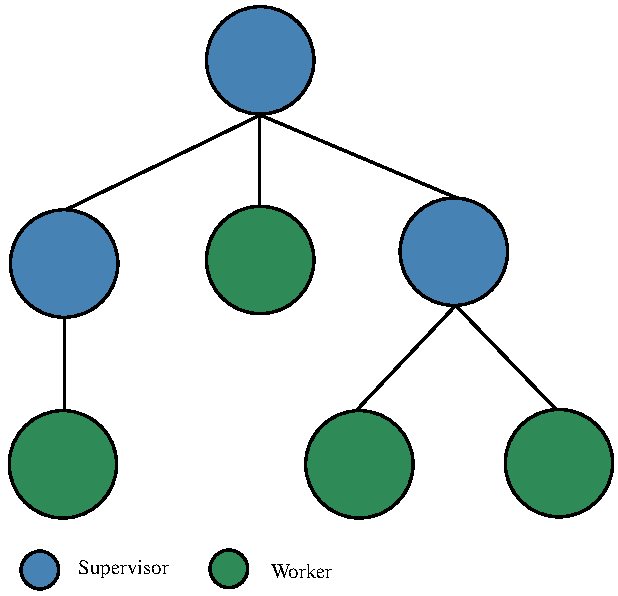
\includegraphics[width=0.5\wholewidth]{supervision-tree}
  \caption[Supervision Tree]{%
    Supervision Tree: Structure of a typical Erlang supervision tree.}
  \label{figure:supervision.tree}
  \normalcaption
\end{figure}

A process as per the supervision tree can either be a supervisor%
\sidenote[-8]{
  \emph{Supervisor}: An Erlang process responsible for creating, terminating,
  monitoring and restarting processes as defined.
}
or a worker%
\sidenote[-5]{
  \emph{Worker}: A worker process in this context is any other process started
  by the supervisor that is not a supervisor itself.
}. Processes that crash are restarted by the supervisor as per its
restart strategy%
\sidenote[-2]{
  \emph{Restart Strategy}: defines how the supervisor should restart
  crashed children.
  \begin{inparaenum}[(i)]
    \iterm{One for one}: Only the crashed process is restarted.
    \iterm{One for all}: All the children under the supervisor are restarted if
    any of the process terminates.
    \iterm{Rest for one}: Similar to one for all, but children restart is based
    on just the first process.
    \iterm{Simple one for one}: Same as one for one, but the children are
    created dynamically.
  \end{inparaenum}
}
. The supervisor also provides several other options such as child
specifications, restart frequency, restart policy and so on to provide
fine grained control on the restart procedure.

\subsection{Behaviours}
\label{section:concepts.behaviours}
Behaviours are commonly used Erlang design patterns. They contain a predefined
set of functions necessary to implement specific design patterns allowing for
quick implementation.

The three main behaviours provided by the OTP library are

\begin{itemize}
    \iterm{gen\_server}: A process that waits for incoming events, performs
    actions based on the events and responds to the request.
    \iterm{gen\_event}: A process that acts as an event manager waiting for
    events to happen and runs specific event handlers based depending on it.
    \iterm{gen\_fsm}: A process that acts as a finite state machine.
\end{itemize}

\subsubsection{gen\_server}
\label{section:gen.server}

gen\_server is based on the typical architecture of client-server model
\citep{reliable.dist.sys}. It supports two types of requests viz, synchronous
calls%
\sidenote{
  \emph{Synchronous calls}: Also called blocking calls, has the caller wait till
  the process can provide a response.
}
and asynchronous calls%
\sidenote[3]{
  \emph{Asynchronous calls}: Also called non-blocking calls, is received by the
  process and handled when it has processed all the messages it had received
  before this request.
}.

It also provides other features such as handling other types of messages (such
as \abbr{TCP}/\abbr{UDP} messages), hot code loading and sending requests to
other processes.

We use gen\_servers to model the roles described in the algorithm.

\subsection{Applications}
\label{section:concepts.applications}
Logical group of components can be glued together to form applications.
This allows us to start and stop the group and define the order for it. It also
makes the code modular, promoting code reusability. Applications have 
well defined roles and Erlang provides convenient ways to
manage them.

\subsection{Releases}
\label{section:concepts.releases}
A release is the complete system packaged for deployment. Erlang provides 
modules necessary to create packages for deploying new code and upgrading
existing code. This helps in rapid development and maintenance of the code.

